%!TEX encoding = UTF-8 Unicode
%!TEX TS-program = xelatex
%
% The first two lines a the top of this file are useful if you use TeXShop.
% They can be deleted or ignored if you are using any other program to compile
% this file.  If you are using TeXShop and do not want to use XeLaTeX, change
% "xelatex" in the second line above to "latex".


%%%%%%%%%%%%%%%%%%%%%%%%%%%%%%%%%%%%%%%
%%%%%                             %%%%%
%%%%% TWPL class file and options %%%%%
%%%%%                             %%%%%
%%%%%%%%%%%%%%%%%%%%%%%%%%%%%%%%%%%%%%%

% In summer 2018, the TWPL formatting guidelines underwent significant revision,
% and the class file's version number was incremented to 1.x from 0.9x. Be sure
% are using the latest version of the TWPL class file. The TWPL class file
% provides for the following options:
%
% [xelatex] to use XeLaTeX (recommended) instead of (pdf)LaTeX (default)
% [linguex] to load the linguex package for linguistics examples
% [gb] to load the gb4e package for linguistics examples
%
% Note that font size and other basic options for the article class are
% already set for you, so you do not need to add any other options.

\documentclass[xelatex,linguex]{TWPL}


%%%%%%%%%%%%%%%%%%%%%%%%%%%%%%%%%%%
%%%%%                         %%%%%
%%%%% Metadata and top matter %%%%%
%%%%%                         %%%%%
%%%%%%%%%%%%%%%%%%%%%%%%%%%%%%%%%%%

% The \articletitle command takes an optional argument inside square
% brackets for an alternative title, which is normally not needed, so
% your \articletitle command will normally look like the following:
%
% \articletitle{Normal paper title with no alternative title} 
%
% However, if the regular title turns out to be too long to fit in the
% header on one line, use the optional argument to provide a shorter
% alternate title (making use of abbreviations, leaving out the subtitle,
% etc.), as in the following:

\articletitle[Title of the paper (on odd pages except page 1, 10pt font, small caps, centred, sentence case)]{Your paper's title in 18pt regular Times New Roman, sentence case} 


% Use both the \author and \affiliation commands, listing the author(s)
% and their affiliation(s). For multiple authors/affiliations, use commas
% to separate three or more, and use "and" before the last one, as follows:
%
% \author{Jane Smith, Chris Thierry, and Alex Yang}
% \affiliation{University of Wherever, Why College, and Nowhere Institute of Technology}

\author{Jane Smith (in 11pt italics)}
\affiliation{University of Wherever (in 11pt italics)}


% Put the contents of your abstract inside the \abstract command:

\abstract{The abstract should be in 10pt font. The paper's title, your name(s), and your affiliation(s) should be set with a 7~cm left margin. There should be one 11pt blank line between the paper title and your name(s), another 11pt blank line between your affiliation(s) and the abstract, and finally another blank 11pt line between the abstract and the header of the first section. The abstract should be fully justified (i.e., flush on both the left and right margins). Conversely, your paper title, names, and affiliations should only be aligned with the left margin. The abstract should not take up more than a third of the page. Try to avoid using special fonts or symbols in your title or abstract as these may not appear correctly on the website and may not be searchable. Most ordinary linguistics diacritics and symbols can be found in the Times New Roman font and thus do not require special fonts.}


% Be sure to set the correct number below for the TWPL volume this article
% belongs to. Volume 41 is the first volume to use the revised 2018 format,
% so your volume number should be at least 41.  Check the TWPL website and/or
% confirm with the editor(s) to verify what number you should use.

\volnum{41}


%%%%%%%%%%%%%%%%%%%%%
%%%%%           %%%%%
%%%%% Main body %%%%%
%%%%%           %%%%%
%%%%%%%%%%%%%%%%%%%%%

% The title, author(s), affiliation(s), abstract, headers, and footers, will
% all be generated automatically, so your document should begin with the first
% section.

\begin{document}

\section{General formatting}

The first paragraph after a main section or sub-section heading should not be indented. Each subsequent paragraph should be indented 0.75~cm. The text should be 11pt Times New Roman, single-spaced, with 0pt spacing before and after each line. As with the abstract, the body of the paper (excluding examples) should be fully justified (i.e., flush with both the left and right margins).

\subsection{Section headings}

Main section headings should be in 11pt bold. Before and after each main section heading there should be a blank 11pt line. The section number should be at the left margin, with the content of the heading indented 0.75~cm from the left margin (not from the section number). There should be no period at the end of the section numbers.

Sub-section headings should be in 11pt italics. Like main section headings, there should be a blank 11pt line before and after each sub-section heading, and the section number should be at the left margin, with the content of the heading indented 0.75~cm, with no period at the end of the section numbers.

Sub-sub-section headings, if needed, should be formatted as described below, separated from the preceding paragraph by a blank 11pt line.

\subsubsection{First sub-sub-section heading.} Sub-sub-section headings should be unnumbered, in 11pt bold, followed by a period, then one space. The body of the sub-sub-section should begin on the same line.

Subsequent paragraphs within the sub-sub-section should be indented 0.75~cm. One blank 11pt line should separate sub-sub-sections from each other. 

\subsubsection{Second sub-sub-section heading.} The next sub-sub-section should start here. In general, sections should never have only one sub-section (and sub-sections shouldn't have only one sub-sub-section). Whenever possible, combine or separate them to fix this problem.

Make sure not to strand section headings at the bottom of a page; they should always be separated from the bottom of the page by at least two lines of body text. % Use \clearpage to do this by hand if needed.

\subsection{Paper body}

The body of the paper should be in 11pt regular font. We strongly recommend using Unicode symbols within Times New Roman when possible. If necessary, you may use special fonts for examples and data, but make sure that these fonts are embedded in the PDF you create. A good way to check that you have done this correctly is to open up the PDF on a computer on which the special font is not installed.

\subsection{Page layout}

The left, right, top, and bottom margins should be 2.54~cm (1 inch). Headers and footers should be set to 1.25~cm from the top and bottom of the page. Make sure the gutter is set to zero. The page size should be set to US letter: 21.59~cm × 27.94~cm (8½″ × 11″), not A4. All these measurements are normally the default in Word.

\subsection{Footnotes}

Footnotes should be numbered, beginning at `1'. A 5~cm line should separate footnotes from the body of the paper (this is the default in Word).\footnote{Footnotes should be in 10pt regular font and fully-justified. Text should have a hanging indent of 0.25~cm so that the number alone is at the left-margin.}  Footnotes should come after the sentence-final punctuation.

At the first use of data in the paper, a footnote should be added that provides the necessary glosses. If the list is too long, it can be given in an appendix.

\subsection{Headers and footers}

Both headers and footers should be set to `different first page'. The first page of the paper will have a blank header and will contain a two-line footer in 10 pt italics. The first line is: Toronto Working Papers in Linguistics (TWPL), Volume \#\#, where \#\# is the Volume number indicated in the Call for Papers to which you are submitting. The second line is © YYYY Author Name(s), where YYYY is the year of publication, and the author(s) name(s) are each listed as given name(s) followed by family name.

Headers should also be set to `different odd and even pages'. Even page headers should contain the name(s) of the author(s), centred and in \textsc{small caps}. Odd page headers (beginning with page~3) should contain the title of the paper, centred and in \textsc{small caps}. (Note that you must still capitalize the first letter of each name, e.g.: \textsc{Barbara Hall Partee}, not \textsc{barbara hall partee}.) If the title would be longer than one line in the header, use an appropriately abbreviated title (for example, remove subtitles and/or abbreviate long words, such as ``\textsc{adv}.'' instead of ``\textsc{advanced}'').

Page numbers should be in 10pt regular font, centred at the bottom of the pages. They should not appear on the first page of the paper.

\section{Data and examples}

The first level of examples should be numbered beginning with (1). These numbers should be flush with the left margin, while the text of the example itself should be indented 0.75~cm. Sub-examples should be listed with letters beginning with `a.', while sub-sub-examples will begin with `i.'. Each level is indented an additional 0.75~cm (see below). Avoid using more than three levels in examples.

\exg. watashi-wa ryokucha-ga suki-desu\\
I-\textsc{top} green.tea-\textsc{nom} like-\textsc{pres.pol}\\
`I like green tea'

\ex. Example
\a. Example
\a. Example
\b. Example

\ex. Example

Leave a blank 11pt line between a block of examples and the main text, and also between examples within a block. Don't leave a blank line between (sub-)sub-examples. Examples should be accompanied by glosses and translations where appropriate, following the Leipzig glossing rules. In particular, use true \textsc{small caps} (i.e., not all caps in a smaller font) to indicate abbreviations of grammatical or functional morphemes. The last line of the example containing the full gloss should be in single quotes.

Graphics demonstrating sign language signs are considered data, and so should be numbered as shown here, and not labelled as figures. Sign language data is given in \textsc{small caps}, with glosses in single quotes when needed. 

\ex. \raisebox{-1in}{\begin{tabular}[t]{@{}c@{}}
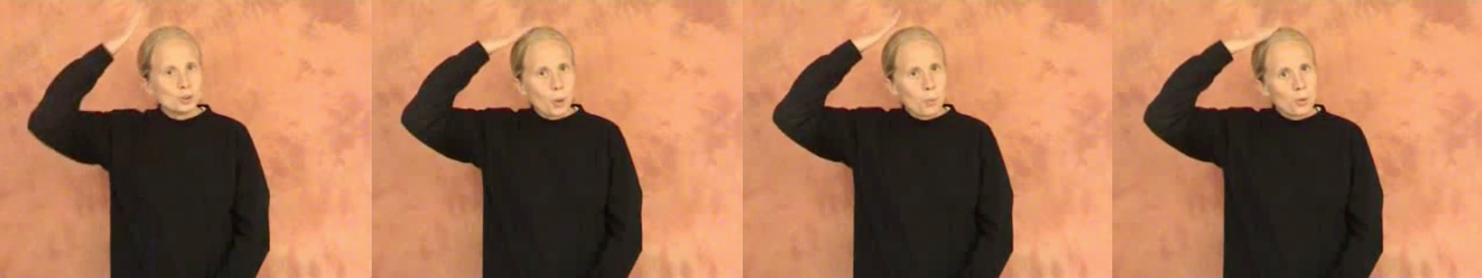
\includegraphics[width=6in]{chapeau.png}\\
\textsc{chapeau} `hat' (Spreadthesign 2012)
\end{tabular}}

Make sure an individual example is not broken up across pages. An example, its gloss, and its translation should be on the same page, but separate examples in the same block can be on different pages. When repeating an earlier example, refer to the first instance of it in the text and then assign it a new number (e.g., ``The example in (2), repeated here as (14), shows\ldots'').

If examples are sourced from another author's work, give the citation including page number where appropriate, either in the main text or to the right of the gloss.

For syntax trees and autosegmental diagrams we strongly recommend using software such as TreeForm or phpSyntaxTree.

\section{Tables and figures}

Make sure that tables and figures fit within the specified margins and are centre-aligned. Tables should use horizontal lines only and avoid vertical lines wherever possible. All tables and figures should be numbered and captioned (10pt font, sentence case). Number tables and figures separately from each other and from the examples in the paper. The caption should appear above tables and below figures. Captions should be separated by one blank 11pt line above and below, and should begin with ``\textbf{Table \#\#.}'' or ``\textbf{Figure \#\#.}'', as appropriate, in bold.

 \begin{figure}
% All floating figures are automatically centred and have [!htp] placement,
% so you do not need to use the \centering command or a placement option.

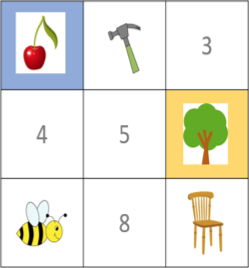
\includegraphics[width=2.1cm]{visual-world.png}

\caption{Visual world display screen}
% Note that figure captions will always be placed below the figure, regardless of
% where the \caption command is placed.
\end{figure}

\begin{table}
% All floating tables are automatically centred and have [!htp] placement,
% so you do not need to use the \centering command or a placement option.

\begin{tabular}{l*{4}{>{$}r<{$}}}
                & \multicolumn{1}{c}{estimate} & \thead{std.~error} & \thead{$z$-value} & \thead{$p$-value} \\
\midrule
\multicolumn{5}{l}{Lexical data (reference level is $g$)}\\
\midrule
(Intercept)     & 0.42673  & 0.10623    & 4.017	    & < 0.001\\
palatalized	    & 0.32117  & 0.21668    & 1.482	    & 0.138\\
cons vs.~vowel  & 0.29839  & 0.07992    & 3.734	    & < 0.001\\
low vs.~non-low	& –0.48934 & 0.12542    & -3.902	& < 0.001\\
\midrule
\end{tabular}

\caption{Fixed effects logistic regression model of lexical data}
% Note that table captions will always be placed below the table, regardless of
% where the \caption command is placed.
\end{table}

\section{Spelling and style}

Canadian, American, and British spellings are all acceptable, as long as you are consistent. For instance, if you spell \emph{flavour} with a <u> you should do the same with \emph{behaviour} and \emph{colour}. A single space should be used after a period and a colon. The numbers one to ten should normally be spelled out, and all others should be given in numerals (unless at the beginning of a sentence, in which case they should be spelled out). For example, ``Eighty-five percent of all speakers aged 18–30\ldots'' Acronyms should be spelled out in full at the first use, followed by the acronym in parentheses. For example, ``According to the Obligatory Contour Principle (OCP)\ldots''.

\subsection{Special formatting}

In-text data from spoken languages should be in italics. Glosses should be in single quotes. For example: ``Discourse marker \emph{like} occurs at a rate of\ldots''; ``The Finnish word \emph{juusto} `cheese' is an example of\ldots''.

Italics should be used for emphasis, terms being defined, and titles of books or journals. Small caps should be used only for grammatical categories, the names of Optimality Theory constraints, or sign language data. Underlining should only be used to highlight part of a word. For example: \emph{abuel\uline{o}}, \emph{abuel\uline{a}}. % The TWPL class automatically loads the ulem package, which provides better underlining with the \uline command. If you use underlining, use \uline rather than the native \underline command.

Use en dash~``–'', not hyphen~``-'' or em dash~``—'', to indicate parentheticals~– like this~– and numerical ranges, including page numbers in references. For example, 120–135, not 120-135. You can enter en dash by pressing Ctrl+``-'' on the numeral pad in Windows, or Option+``-'' on a Mac.  % In LaTeX, you can use the code -- (two hyphens) to get an en dash, without having to type it directly. However, this file allows for some direct Unicode input, so you can type – directly here as well.

\section{In-text citations}

Citations follow the Association Canadienne de Linguistique / Canadian Linguistic Association (ACL/CLA) style for the \emph{Canadian Journal of Linguistics}. Notably, this means:

\begin{enumerate}\setlength\itemsep{-0.75ex}
\item No comma between the author and the year
\item A space between the colon and the page number
\item A comma between different citations by the same author
\item A semi-colon between citations by different authors
\item For two authors, give both names and no ampersand (\&)
\item For more than two authors, give the first name followed by ``et al.''
\item Citations grouped by author and listed chronologically by each author's first citation
\end{enumerate}

Examples are given here:

\begin{quote}
``Indeed, in the modern languages phonetic conditioning is typically absent for the vast majority of mutation cases.'' \citep[2811]{Hannahs2010} % Note the use of \citep's optional argument for page numbers. This optional argument works for any of the \cite commands (\citet, \citealt, etc.)

Coronals have been shown to hold a special status among consonants \citep{Kiparsky1985, AveryRice1989}.

Referring expressions are interpreted through simultaneous integration of the common ground and one's egocentric knowledge \citep{HellerEtal2016}.

The second highest status group shows the greatest gender differences \citep{Labov1966, Labov2001, Wolfram1971, Eckert1999}. % The TWPL class file will put citations in the order given, so please make sure they are correctly grouped and ordered as described by the style guide.

\end{quote}

When making author's names possessive, the possessive morpheme should come after the name and before the year (e.g., ``\citeposs{Reuland2011} taxonomy''). % Note the use of the dedicated \citeposs command in the TWPL class file. This can also be built up compositionally with \citeauthor and \citeyear if needed, for example, to say ``\citeauthor{Reuland2011}'s innovative \citeyear{Reuland2011} taxonomy''.

\section{Acknowledgments, references, and appendices}

\subsection{Acknowledgments}

Acknowledgments go at the end of the paper, before the references. Leave two blank 11pt lines between the final paragraph of the main text and the acknowledgements. The header ``\textbf{Acknowledgments}'' should be in bold 11pt. The acknowledgments themselves should start on the same line as the header.

At the end of the acknowledgments, or the end of the paper if you don't have acknowledgments, leave two 11pt blank lines and then the word ``\textbf{References}'' in bold 11pt font. Below that, leave one 11pt blank line.

\subsection{References}

References should be single-spaced, with no blank lines between entries, fully justified with both margins. The second and successive lines of individual reference entries should be indented 0.75~cm (i.e., a hanging indent). References should be in 11pt font like the main text.

The format for references should follow the ACL/CLA style for the \emph{Canadian Journal of Linguistics}.

\subsection{Appendices}

Appendices follow the references. They should be given a representative title. If you have only one appendix, it shouldn't be lettered~– simply title it ``\textbf{Appendix: Title}''. If you have more than one, they should be lettered sequentially: \textbf{Appendix A}, \textbf{Appendix B}, etc. At the end of your references, leave two blank 11pt lines and then the appendix heading in bold 11pt font. Leave a blank 11pt line between the heading and the body of the appendix. If you have multiple appendices, leave two blank 11pt lines between the end of one and the title heading of the other. All other guidelines (font size, margins, etc.) remain the same as in the body of the paper.


%%%%%%%%%%%%%%%%%%%%%%%%%%%%%%%%%%%%%%%
%%%%%                             %%%%%
%%%%% Acknowledgements (optional) %%%%%
%%%%%                             %%%%%
%%%%%%%%%%%%%%%%%%%%%%%%%%%%%%%%%%%%%%%

% Put acknowledgments here. Delete the following if you have no acknowledgements.
\vspace{22pt}\noindent\textbf{Acknowledgements.} Any acknowledgments go here.


%%%%%%%%%%%%%%%%%%%%%%%%%%%%%%%%%%%%%%%%%%%%
%%%%%                                  %%%%%
%%%%% Automated references with BibTeX %%%%%
%%%%%                                  %%%%%
%%%%%%%%%%%%%%%%%%%%%%%%%%%%%%%%%%%%%%%%%%%%

% The following are some extra sample references that are loaded by BibTeX to
% demonstrate various aspects of the bibliographic format. You should not need
% this line for your own article, so delete it or comment it out.
\nocite{Armon1996, Blevins2008a, Blevins2008b, Goldsmith1995, Kahnemuyipour2001, NakayamaArchibald2005, Reinhart1976, Rice1997, Writer1999, WriterToAppear}

% TWPL references follow the formatting for the Canadian Journal of Linguistics, which
% is given in the RCL.bst file, loaded below.  If you are inputting your references
% directly, rather than using BibTeX, you should delete or comment out this line and
% follow the directions below.
\bibliographystyle{RCL.bst}

% The sample references used here are from the SampleRefs.bib file, loaded below, but
% you should use your own personal .bib file here.  If you are inputting your references
% directly, rather than using BibTeX, you should delete or comment out this line and
% follow the directions below.
\bibliography{SampleRefs}


%%%%%%%%%%%%%%%%%%%%%%%%%%%%%%%%%%%%%%%%%%%%%%%%%%%%%%%%%%%%%%%%
%%%%%                                                      %%%%%
%%%%% Entering references directly instead of using BibTeX %%%%%
%%%%%                                                      %%%%%
%%%%%%%%%%%%%%%%%%%%%%%%%%%%%%%%%%%%%%%%%%%%%%%%%%%%%%%%%%%%%%%%

% Uncomment the following two lines, and then enter your references as in the examples
% below. Be sure to end the hangparas environment with a \end{hangparas} command.
%\vspace{11pt}\section*{References}
%\begin{hangparas}{0.75cm}{1}

%Armon-Loten, Sharon. 1996. What Hebrew early verbs teach us about root infinitives. In \emph{Proceedings of the Groningen Assembly on Language Acquisition (GALA) 1995}, ed. Charlotte Koster and Frank Wijnen, 77–86. Groningen: Center for Language and Cognition. 
%
%Avery, Peter, and Keren Rice. 1989. Segment structure and coronal underspecification. Phonology 6(2): 179–200.
%
%Blevins, Juliette. 2008a. Natural and unnatural sound patterns: A pocket field guide. In \emph{Naturalness and iconicity in language}, ed. Klaas Willems and Ludovic De Cuypere, 121–148. Amsterdam: John Benjamins.
%
%Blevins, Juliette. 2008b. Phonetic explanation without compromise. \emph{Diachronica} 25: 1–19.
%
%Eckert, Penelope. 1999. \emph{Variation as social practice}. Oxford: Blackwell.
%
%Goldsmith, John, ed. 1995. \emph{The handbook of phonological theory}. Oxford: Blackwell.
%
%Hannahs, S. J. 2010. Celtic mutations. In \emph{The Blackwell companion to phonology}, ed. Colin J. Ewen, Keren Rice, Elizabeth Hume, and Marc van Oostendorp, vol. 5, 2807–2830. Malden, MA: Wiley-Blackwell.
%
%Heller, Daphna, Christopher Parisien, and Suzanne Stevenson. 2016. Perspective-taking behaviour as the probabilistic weighing of multiple domains. \emph{Cognition} 149: 104–120.
%
%Kahnemuyipour, Arsalan. 2001. On \emph{wh}-questions in Persian. \emph{Canadian Journal of Linguistics} 46(1): 41–61.
%
%Kiparsky, Paul. 1985. Some consequences of Lexical Phonology. \emph{Phonology Handbook} 2: 85–138.
%
%Labov, William. 1966. \emph{The social stratification of English in New York City}. Washington, DC: Center for Applied Linguistics.
%
%Labov, William. 2001. \emph{Principles of linguistic change. Volume II: Social factors}. Oxford: Blackwell. 
%
%Nakayama, Mariko, and John Archibald. 2005. Eye-tracking and interlingual homographs: Evidence for non-selective access to the bilingual lexicon. Paper presented at the annual meeting of the Canadian Linguistic Association, London, ON.
%
%Reinhart, Tanya. 1976. The syntactic domain of anaphora. Doctoral dissertation, Massachusetts Institute of Technology.
%
%Reuland, Eric. 2011. \emph{Anaphora and language design}. Cambridge, MA: MIT Press.
%
%Rice, Keren. 1997. Japanese NC clusters and the redundancy of postnasal voicing. \emph{Linguistic Inquiry} 28(1): 541–551.
%
%Wolfram, Walt. 1971. \emph{Black-white speech relationships}. Washington, DC: Center for Applied Linguistics. 
%
%Writer, Wanda. 1999. Title of unpublished manuscript. Ms., University Name.
%
%Writer, Wei Li. To appear. Title of article. \emph{Journal}. 

%\end{hangparas}


%%%%%%%%%%%%%%%%%%%%%%
%%%%%            %%%%%
%%%%% Appendices %%%%%
%%%%%            %%%%%
%%%%%%%%%%%%%%%%%%%%%%

\vspace{11pt}\section*{Appendix A: Sample acceptability judgment task survey}

Please rate these words with the numbers 1–5, using the explanations for each number given here:

\bigskip

\noindent
\begin{tabular}{@{}l@{~}l@{}}
1: & I've never seen or heard a word like this. I don't think anyone would ever say it.\\
2: & I'm not sure if I would say a word like this or not.\\
3: & I think this word is perfectly fine.\\
\end{tabular}

\bigskip

\begin{tabular}{@{}l@{\quad}c@{\qquad\qquad}c@{\qquad\qquad}cc@{}}
mhíogha & 1 & 2 & 3 & \\
\\
\multicolumn{5}{@{}l@{}}{If this word isn't good, can you explain what's bad about it?}\\
\\
bheirsil & 1 & 2 & 3 & \\
\\
\multicolumn{5}{@{}l@{}}{If this word isn't good, can you explain what's bad about it?}\\
\\
ghaonra & 1 & 2 & 3 & \\
\\
\multicolumn{5}{@{}l@{}}{If this word isn't good, can you explain what's bad about it?}\\
\end{tabular}

\vspace{11pt}

\section*{Appendix B:  List of experimental items}

\noindent\hspace*{\fill}
\begin{tabular}{cccccc}
 & d & g & filler p & filler b & filler m\\
\midrule
High front & dhís & ghíg & phíbhan & bhíb & mhíogha\\
 & dhímh & ghíom & phíogha & bhís & mhíbhan\\
\midrule
Mid front & dhelan & ghaonra & pheilimh & bheirsil & mheg\\
 & dhen & gherre & pheirb & bherre & mheirna\\
\midrule
Low central & dhalcas & ghaib & pheanat & bhachú & mhean\\
 & danal & ghailadh & phallibh & bheanat & mhallibh\\
\midrule
\end{tabular}
\hspace*{\fill}

\end{document}
